% (find-LATEX "2020-1-C3-aprox-2a-ordem-R2.tex")
% (defun c () (interactive) (find-LATEXsh "lualatex -record 2020-1-C3-aprox-2a-ordem-R2.tex" :end))
% (defun D () (interactive) (find-pdf-page      "~/LATEX/2020-1-C3-aprox-2a-ordem-R2.pdf"))
% (defun d () (interactive) (find-pdftools-page "~/LATEX/2020-1-C3-aprox-2a-ordem-R2.pdf"))
% (defun e () (interactive) (find-LATEX "2020-1-C3-aprox-2a-ordem-R2.tex"))
% (defun u () (interactive) (find-latex-upload-links "2020-1-C3-aprox-2a-ordem-R2"))
% (defun v () (interactive) (find-2a '(e) '(d)) (g))
% (find-pdf-page   "~/LATEX/2020-1-C3-aprox-2a-ordem-R2.pdf")
% (find-sh0 "cp -v  ~/LATEX/2020-1-C3-aprox-2a-ordem-R2.pdf /tmp/")
% (find-sh0 "cp -v  ~/LATEX/2020-1-C3-aprox-2a-ordem-R2.pdf /tmp/pen/")
%   file:///home/edrx/LATEX/2020-1-C3-aprox-2a-ordem-R2.pdf
%               file:///tmp/2020-1-C3-aprox-2a-ordem-R2.pdf
%           file:///tmp/pen/2020-1-C3-aprox-2a-ordem-R2.pdf
% http://angg.twu.net/LATEX/2020-1-C3-aprox-2a-ordem-R2.pdf
% (find-LATEX "2019.mk")

% «.scans»		(to "scans")
% «.videos»		(to "videos")
% «.exercicio-1»	(to "exercicio-1")
% «.exercicio-2»	(to "exercicio-2")
% «.exercicio-2b»	(to "exercicio-2b")
%
\documentclass[oneside,12pt]{article}
\usepackage[colorlinks,citecolor=DarkRed,urlcolor=DarkRed]{hyperref} % (find-es "tex" "hyperref")
\usepackage{amsmath}
\usepackage{amsfonts}
\usepackage{amssymb}
\usepackage{pict2e}
\usepackage[x11names,svgnames]{xcolor} % (find-es "tex" "xcolor")
%\usepackage{colorweb}                 % (find-es "tex" "colorweb")
%\usepackage{tikz}
%
% (find-dn6 "preamble6.lua" "preamble0")
%\usepackage{proof}   % For derivation trees ("%:" lines)
%\input diagxy        % For 2D diagrams ("%D" lines)
%\xyoption{curve}     % For the ".curve=" feature in 2D diagrams
%
\usepackage{edrx15}               % (find-LATEX "edrx15.sty")
\input edrxaccents.tex            % (find-LATEX "edrxaccents.tex")
\input edrxchars.tex              % (find-LATEX "edrxchars.tex")
\input edrxheadfoot.tex           % (find-LATEX "edrxheadfoot.tex")
\input edrxgac2.tex               % (find-LATEX "edrxgac2.tex")
%
%\usepackage[backend=biber,
%   style=alphabetic]{biblatex}            % (find-es "tex" "biber")
%\addbibresource{catsem-slides.bib}        % (find-LATEX "catsem-slides.bib")
%
% (find-es "tex" "geometry")
\usepackage[a6paper, landscape,
            top=1.5cm, bottom=.25cm, left=1cm, right=1cm, includefoot
           ]{geometry}
%
\begin{document}

\catcode`\^^J=10
\directlua{dofile "dednat6load.lua"}  % (find-LATEX "dednat6load.lua")

% «defs»  (to ".defs")
% (find-LATEX "edrx15.sty" "colors-2019")
\long\def\ColorRed   #1{{\color{Red1}#1}}
\long\def\ColorViolet#1{{\color{MagentaVioletLight}#1}}
\long\def\ColorViolet#1{{\color{Violet!50!black}#1}}
\long\def\ColorGreen #1{{\color{SpringDarkHard}#1}}
\long\def\ColorGreen #1{{\color{SpringGreenDark}#1}}
\long\def\ColorGreen #1{{\color{SpringGreen4}#1}}
\long\def\ColorGray  #1{{\color{GrayLight}#1}}
\long\def\ColorGray  #1{{\color{black!30!white}#1}}
\long\def\ColorBrown #1{{\color{Brown}#1}}
\long\def\ColorBrown #1{{\color{brown}#1}}

\long\def\ColorShort #1{{\color{SpringGreen4}#1}}
\long\def\ColorLong  #1{{\color{Red1}#1}}

\def\frown{\ensuremath{{=}{(}}}
\def\True {\mathbf{V}}
\def\False{\mathbf{F}}

\def\drafturl{http://angg.twu.net/LATEX/2020-1-C2.pdf}
\def\drafturl{http://angg.twu.net/2020.1-C2.html}
\def\draftfooter{\tiny \href{\drafturl}{\jobname{}} \ColorBrown{\shorttoday{} \hours}}


%  _____ _ _   _                               
% |_   _(_) |_| | ___   _ __   __ _  __ _  ___ 
%   | | | | __| |/ _ \ | '_ \ / _` |/ _` |/ _ \
%   | | | | |_| |  __/ | |_) | (_| | (_| |  __/
%   |_| |_|\__|_|\___| | .__/ \__,_|\__, |\___|
%                      |_|          |___/      
%
% «title»  (to ".title")
% (c3m201aprox2aop 1 "title")
% (c3m201aprox2aoa   "title")

\thispagestyle{empty}

\begin{center}

\vspace*{1.2cm}

{\bf \Large Cálculo 3 - 2020.1}

\bsk

Aula 19: aproximações de 2ª ordem em $\R^2$

\bsk

Eduardo Ochs - RCN/PURO/UFF

\url{http://angg.twu.net/2020.1-C3.html}

\end{center}

\newpage

{\bf Introdução}

\ssk

Leia bem por alto o início do capítulo 10 do Bortolossi...

Hoje nós vamos {\sl começar} a entender como encontrar

máximos e mínimos locais de funções de duas variáveis.

% (find-books "__analysis/__analysis.el" "bortolossi")
% (find-bortolossi10page (+ -350 351) "10. Máximos e mínimos de funções de várias variáveis")


\newpage

{\bf Grau de um polinômio em duas variáveis}

% (find-latexscan-links "C3" "20201125_114928_poli_grau_5")
% (find-xpdf-page "~/LATEX/2020-1-C3/20201125_114928_poli_grau_5.pdf")
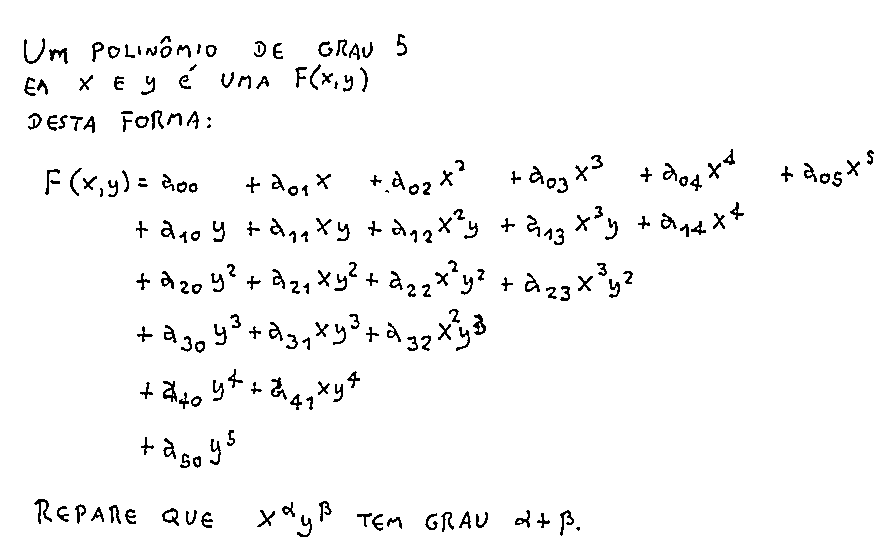
\includegraphics[width=11cm]{2020-1-C3/20201125_114928_poli_grau_5.pdf}

\newpage

{\bf Aproximação de 2a ordem}

% (find-latexscan-links "C3" "20201125_115033_aprox_2a_ordem")
% (find-xpdf-page "~/LATEX/2020-1-C3/20201125_115033_aprox_2a_ordem.pdf")
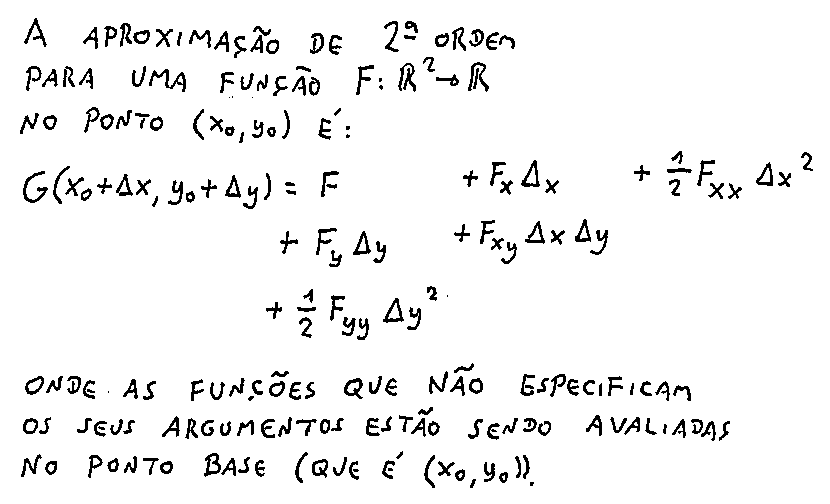
\includegraphics[width=11cm]{2020-1-C3/20201125_115033_aprox_2a_ordem.pdf}

\newpage

% «exercicio-1»  (to ".exercicio-1")
% (c3m201aprox2aop 5 "exercicio-1")
% (c3m201aprox2ao    "exercicio-1")

{\bf Exercício 1}

% (find-latexscan-links          "C3" "20201125_115134_exerc_1")
% (find-xpdf-page   "~/LATEX/2020-1-C3/20201125_115134_exerc_1.pdf")
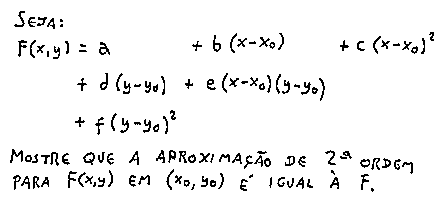
\includegraphics[width=11cm]{2020-1-C3/20201125_115134_exerc_1.pdf}

\newpage

% «exercicio-2»  (to ".exercicio-2")
% (c3m201aprox2aop 6 "exercicio-2")
% (c3m201aprox2ao    "exercicio-2")

{\bf Exercício 2}

% (find-latexscan-links "C3" "20201125_115243_exerc_2a")
% (find-xpdf-page "~/LATEX/2020-1-C3/20201125_115243_exerc_2a.pdf")
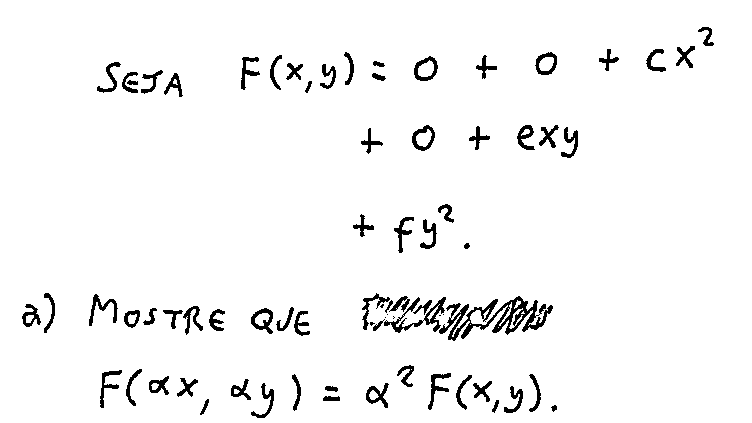
\includegraphics[width=11cm]{2020-1-C3/20201125_115243_exerc_2a.pdf}

\newpage

% «exercicio-2b»  (to ".exercicio-2b")
% (c3m201aprox2aop 7 "exercicio-2b")
% (c3m201aprox2ao    "exercicio-2b")

{\bf Exercício 2 (item b)}

% (find-latexscan-links "C3" "20201125_115407_exerc_2b")
% (find-xpdf-page "~/LATEX/2020-1-C3/20201125_115407_exerc_2b.pdf")
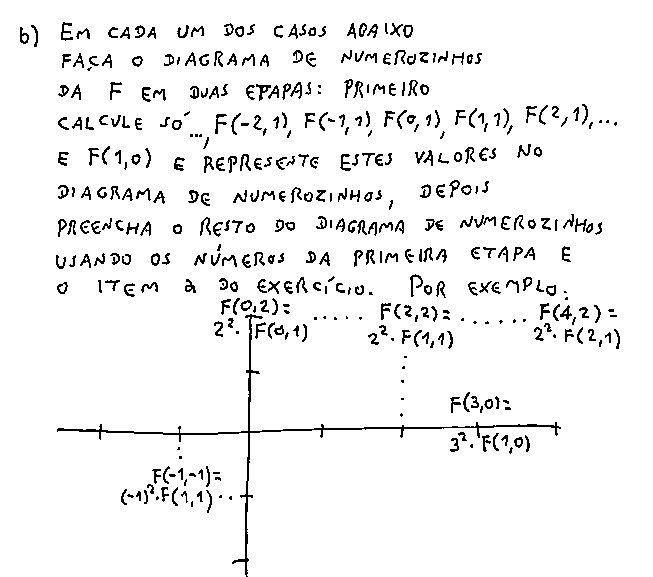
\includegraphics[height=7cm]{2020-1-C3/20201125_115407_exerc_2b.pdf}

\newpage

{\bf Exercício 2 (item b, casos 1, 2, 3, 4)}

% (find-latexscan-links "C3" "20201125_120703_exerc_2b_casos_1234")
% (find-xpdf-page "~/LATEX/2020-1-C3/20201125_120703_exerc_2b_casos_1234.pdf")
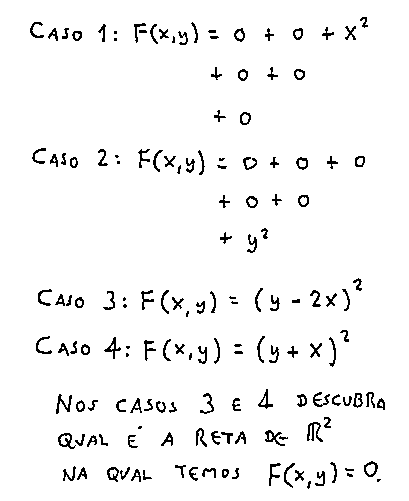
\includegraphics[height=7cm]{2020-1-C3/20201125_120703_exerc_2b_casos_1234.pdf}

\newpage

{\bf Exercício 2 (item b, caso 5)}

% (find-latexscan-links "C3" "20201125_120744_exerc_2b_caso_5")
% (find-xpdf-page "~/LATEX/2020-1-C3/20201125_120744_exerc_2b_caso_5.pdf")
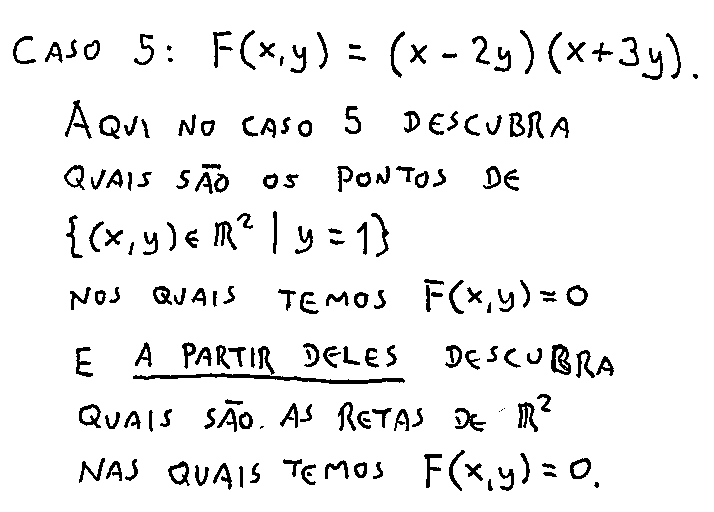
\includegraphics[height=7cm]{2020-1-C3/20201125_120744_exerc_2b_caso_5.pdf}



% %L dofile "edrxtikz.lua"  -- (find-LATEX "edrxtikz.lua")
% %L dofile "edrxpict.lua"  -- (find-LATEX "edrxpict.lua")
% \pu

%\printbibliography

\end{document}

%  ____                      
% / ___|  ___ __ _ _ __  ___ 
% \___ \ / __/ _` | '_ \/ __|
%  ___) | (_| (_| | | | \__ \
% |____/ \___\__,_|_| |_|___/
%                            
% «scans»  (to ".scans")

 (eepitch-shell)
 (eepitch-kill)
 (eepitch-shell)
# (find-fline "~/2020.1-C3/")
# (find-fline "/tmp/qc3/")
# (find-fline "/tmp/c3mt2/")
# (find-fline "~/LATEX/2020-1-C3/")
cd /tmp/qc3/
cd /tmp/
f () { rm -fv $1.png $1.pdf; djvuize $1.pdf }
f () { rm -fv $1.png $1.pdf; djvuize WHITEBOARDOPTS="-m 0.5" $1.pdf; xpdf $1.pdf }
f () { rm -fv $1.png $1.pdf; djvuize WHITEBOARDOPTS="-m 0.25" $1.pdf; xpdf $1.pdf }
f () { cp -fv $1.png $1.pdf       ~/2020.1-C3/ }
f () { cp -fv        $1.pdf ~/LATEX/2020-1-C3/ }
f () { cp -fv $1.png $1.pdf       ~/2020.1-C3/
       cp -fv        $1.pdf ~/LATEX/2020-1-C3/
     }
f () { echo "% (find-latexscan-links \"C3\" \"$1\")" }

f 20201125_C3_mt2

f 20201125_114928_poli_grau_5
f 20201125_115033_aprox_2a_ordem
f 20201125_115134_exerc_1
f 20201125_115243_exerc_2a
f 20201125_115407_exerc_2b
f 20201125_120703_exerc_2b_casos_1234
f 20201125_120744_exerc_2b_caso_5



% «videos»  (to ".videos")
% (find-ssr-links "2020_C3_2020nov25_aprox_2a_ordem" "c3a2o")

 (eepitch-shell)
 (eepitch-kill)
 (eepitch-shell)
cp -v  ~/LATEX/2020-1-C3-aprox-2a-ordem-R2.pdf /tmp/
cd /tmp/
xournalpp 2020-1-C3-aprox-2a-ordem-R2.pdf





%  __  __       _        
% |  \/  | __ _| | _____ 
% | |\/| |/ _` | |/ / _ \
% | |  | | (_| |   <  __/
% |_|  |_|\__,_|_|\_\___|
%                        
% <make>

 (eepitch-shell)
 (eepitch-kill)
 (eepitch-shell)
# (find-LATEXfile "2019planar-has-1.mk")
make -f 2019.mk STEM=2020-1-C3-aprox-2a-ordem-R2 veryclean
make -f 2019.mk STEM=2020-1-C3-aprox-2a-ordem-R2 pdf

% Local Variables:
% coding: utf-8-unix
% ee-tla: "c3m201aprox2ao"
% End:
